\documentclass{beamer}
\usepackage[utf8]{inputenc}

\usepackage{amsmath}
\usepackage{graphicx}
\usepackage{url}
\usepackage{fancyvrb}
\usepackage{xcolor}

\usetheme{Antibes}
\usecolortheme{whale}
\usepackage{lmodern}

\usepackage{listings}
\usepackage{color}

\definecolor{codegreen}{rgb}{0,0.6,0}
\definecolor{codegray}{rgb}{0.5,0.5,0.5}
\definecolor{codepurple}{rgb}{0.58,0,0.82}
\definecolor{backcolour}{rgb}{0.95,0.95,0.92}

\mode<presentation>

\definecolor{orange}{HTML}{BC2E07}

\usepackage{hyperref}
\hypersetup{
    colorlinks,
    linkcolor=orange,
    urlcolor=blue
}

\lstdefinestyle{mystyle}{
    language=C++,
    basicstyle=\ttfamily\footnotesize,
    backgroundcolor=\color{backcolour},
    commentstyle=\color{codegreen},
    keywordstyle=\color{magenta},
    numberstyle=\tiny\color{codegray},
    stringstyle=\color{codepurple},
    breakatwhitespace=false,
    breaklines=true,
    captionpos=b,
    keepspaces=true,
    numbers=left,
    numbersep=5pt,
    showspaces=false,
    showstringspaces=false,
    showtabs=false,
    tabsize=2
}

\title{Lab \# 9: Lab Practice}
\subtitle{EC-102 -- Computer Systems and Programming}

\author{Usama Wajhi}
\institute{School of Mechanical and Manufacturing Engineering (SMME), \\ National University of Sciences and Technology (NUST)}
\date{\today}

\begin{document}
\begin{frame}
    \titlepage
\end{frame}


\begin{frame}
    \frametitle{Outline}
        \tableofcontents
\end{frame}
\begin{frame}
    \frametitle{Problem : 1}
    \section{Problem : 1}
\begin{LARGE}
Write a program to draw a Pyramid, program must ask the user about the height of Pyramid.
\end{LARGE}

    

\end{frame}
\begin{frame}
    \frametitle{Problem : 2}
    \section{Problem : 2}
    Write a program to draw an empty diamond, program must ask the user about the height of diamond.
    \begin{figure}
                \centering
                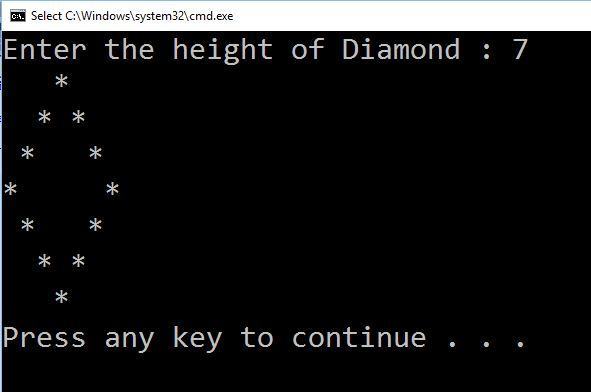
\includegraphics[scale=0.4]{out1}
    \end{figure}

\end{frame}

\end{document}